\documentclass{article}
\usepackage{amsmath}
\usepackage{setspace}
\usepackage{adjustbox}
\usepackage{graphicx}
\usepackage{float}
\usepackage{multicol}
\usepackage{hyperref}
\usepackage{subfig}
\usepackage{wrapfig}
\usepackage{xcolor}
\usepackage{tabularray}
\usepackage{sidecap}
%\usepackage{natbib,url}
\usepackage[backend=biber,style=numeric,maxnames =2,giveninits = true]{biblatex}
\addbibresource{journal_abbreviations.bib}
\addbibresource{References.bib}
\usepackage[margin = 1in]{geometry}
%\bibliographystyle{abbrv}
\DeclareBibliographyDriver{std}{%
  \usebibmacro{bibindex}%
  \usebibmacro{begentry}%
  \usebibmacro{author/editor+others/translator+others}%
  \setunit{\labelnamepunct}\newblock
  %\usebibmacro{title}%
    %\newunit\newblock
  \usebibmacro{journal}
  \newunit\newblock
  \usebibmacro{date}%
  \newunit\newblock
\usebibmacro{finentry}}

\DeclareBibliographyDriver{stdbook}{%
  \usebibmacro{bibindex}%
  \usebibmacro{begentry}%
  \usebibmacro{author/editor+others/translator+others}%
  \setunit{\labelnamepunct}\newblock
  %\usebibmacro{title}%
  \usebibmacro{title}
  \newunit\newblock
  \usebibmacro{date}%
  \newunit\newblock
\usebibmacro{finentry}}

\DeclareBibliographyAlias{article}{std}
\DeclareBibliographyAlias{book}{stdbook}
\DeclareBibliographyAlias{misc}{stdbook}
\AtBeginBibliography{\small}
\definecolor{gray_c}{rgb}{0.745, 0.898, 0.898}
\definecolor{gray_h}{rgb}{0.43, 0.72, 0.72}

\def\epo{\epsilon\rightarrow 0}
\def\lb{\left(}
\def\rb{\right)}
\def\ls{\left[ \vphantom]}
\def\rs{\right] }
\def\ep{\epsilon}

\title{Direct simulation of ocean-ice coupling in icy moons}
\author{Tobias Oliver}
\date{}

\begin{document}
\newcommand{\citep}[1]{\cite{#1}}
\maketitle
\section{Summary}
I propose to study to processes important to the interaction between the ocean and ice on the ``ocean worlds'' of the Jovian and Saturnian system. Forward, numerical simulations will be used to better constrain the dynamics of the sub-surface oceans on these planets. A focus is placed on two models that will couple ocean dynamics to the ice, so that surface observations from the upcoming \textit{Europa Clipper} and \textit{JUICE} missions can be used to predict ocean dynamics.
First, I will study a conjugate heat transfer model in which the surface response to underlying convection is directly simulated. No prior simulations of this type exist in the planetary literature. Second, I will investigate a double diffusive model, involving the coupled dynamics of solutal and thermal buoyancy. This process is thought to be particularly important near the ocean-ice interface where melting ice releases cold, fresh water into the underlying ocean.
\section{Intellectual Merit}
The solar system contains a number of icy bodies, many of which are thought to be ``ocean worlds,'' that may be suitable candidates for the habitability of life.
The primary objective of NASA's \textit{Europa Clipper} (EC) (\cite{pC14_JUICE}) and ESA's \textit{Jupiter Icy Moons Explorer} (JUICE)\citep{oG13} missions is to investigate Europa, Ganymede, and Callisto, three Jovian satellites believed to be ocean worlds. Each is expected contain salty, liquid oceans underneath thin icy shells \citep{rP99,fN16}, and both EC and JUICE aim to determine whether these bodies contain necessary conditions for life\citep{tB24}. Figure \ref{f:pic}(a) illustrates a proposed structure.
The sub-surface oceans link the solid cores of these moons to their icy exteriors, and are therefore expected to play an important role in the transport of heat and chemicals to their surfaces \citep{kS20}. 

\begin{wrapfigure}{R}{0.6\textwidth}
	\begin{center}
		\subfloat[][]{\includegraphics[width=0.25\textwidth]{figures/europa_ice}}
		\quad
	\subfloat[][]{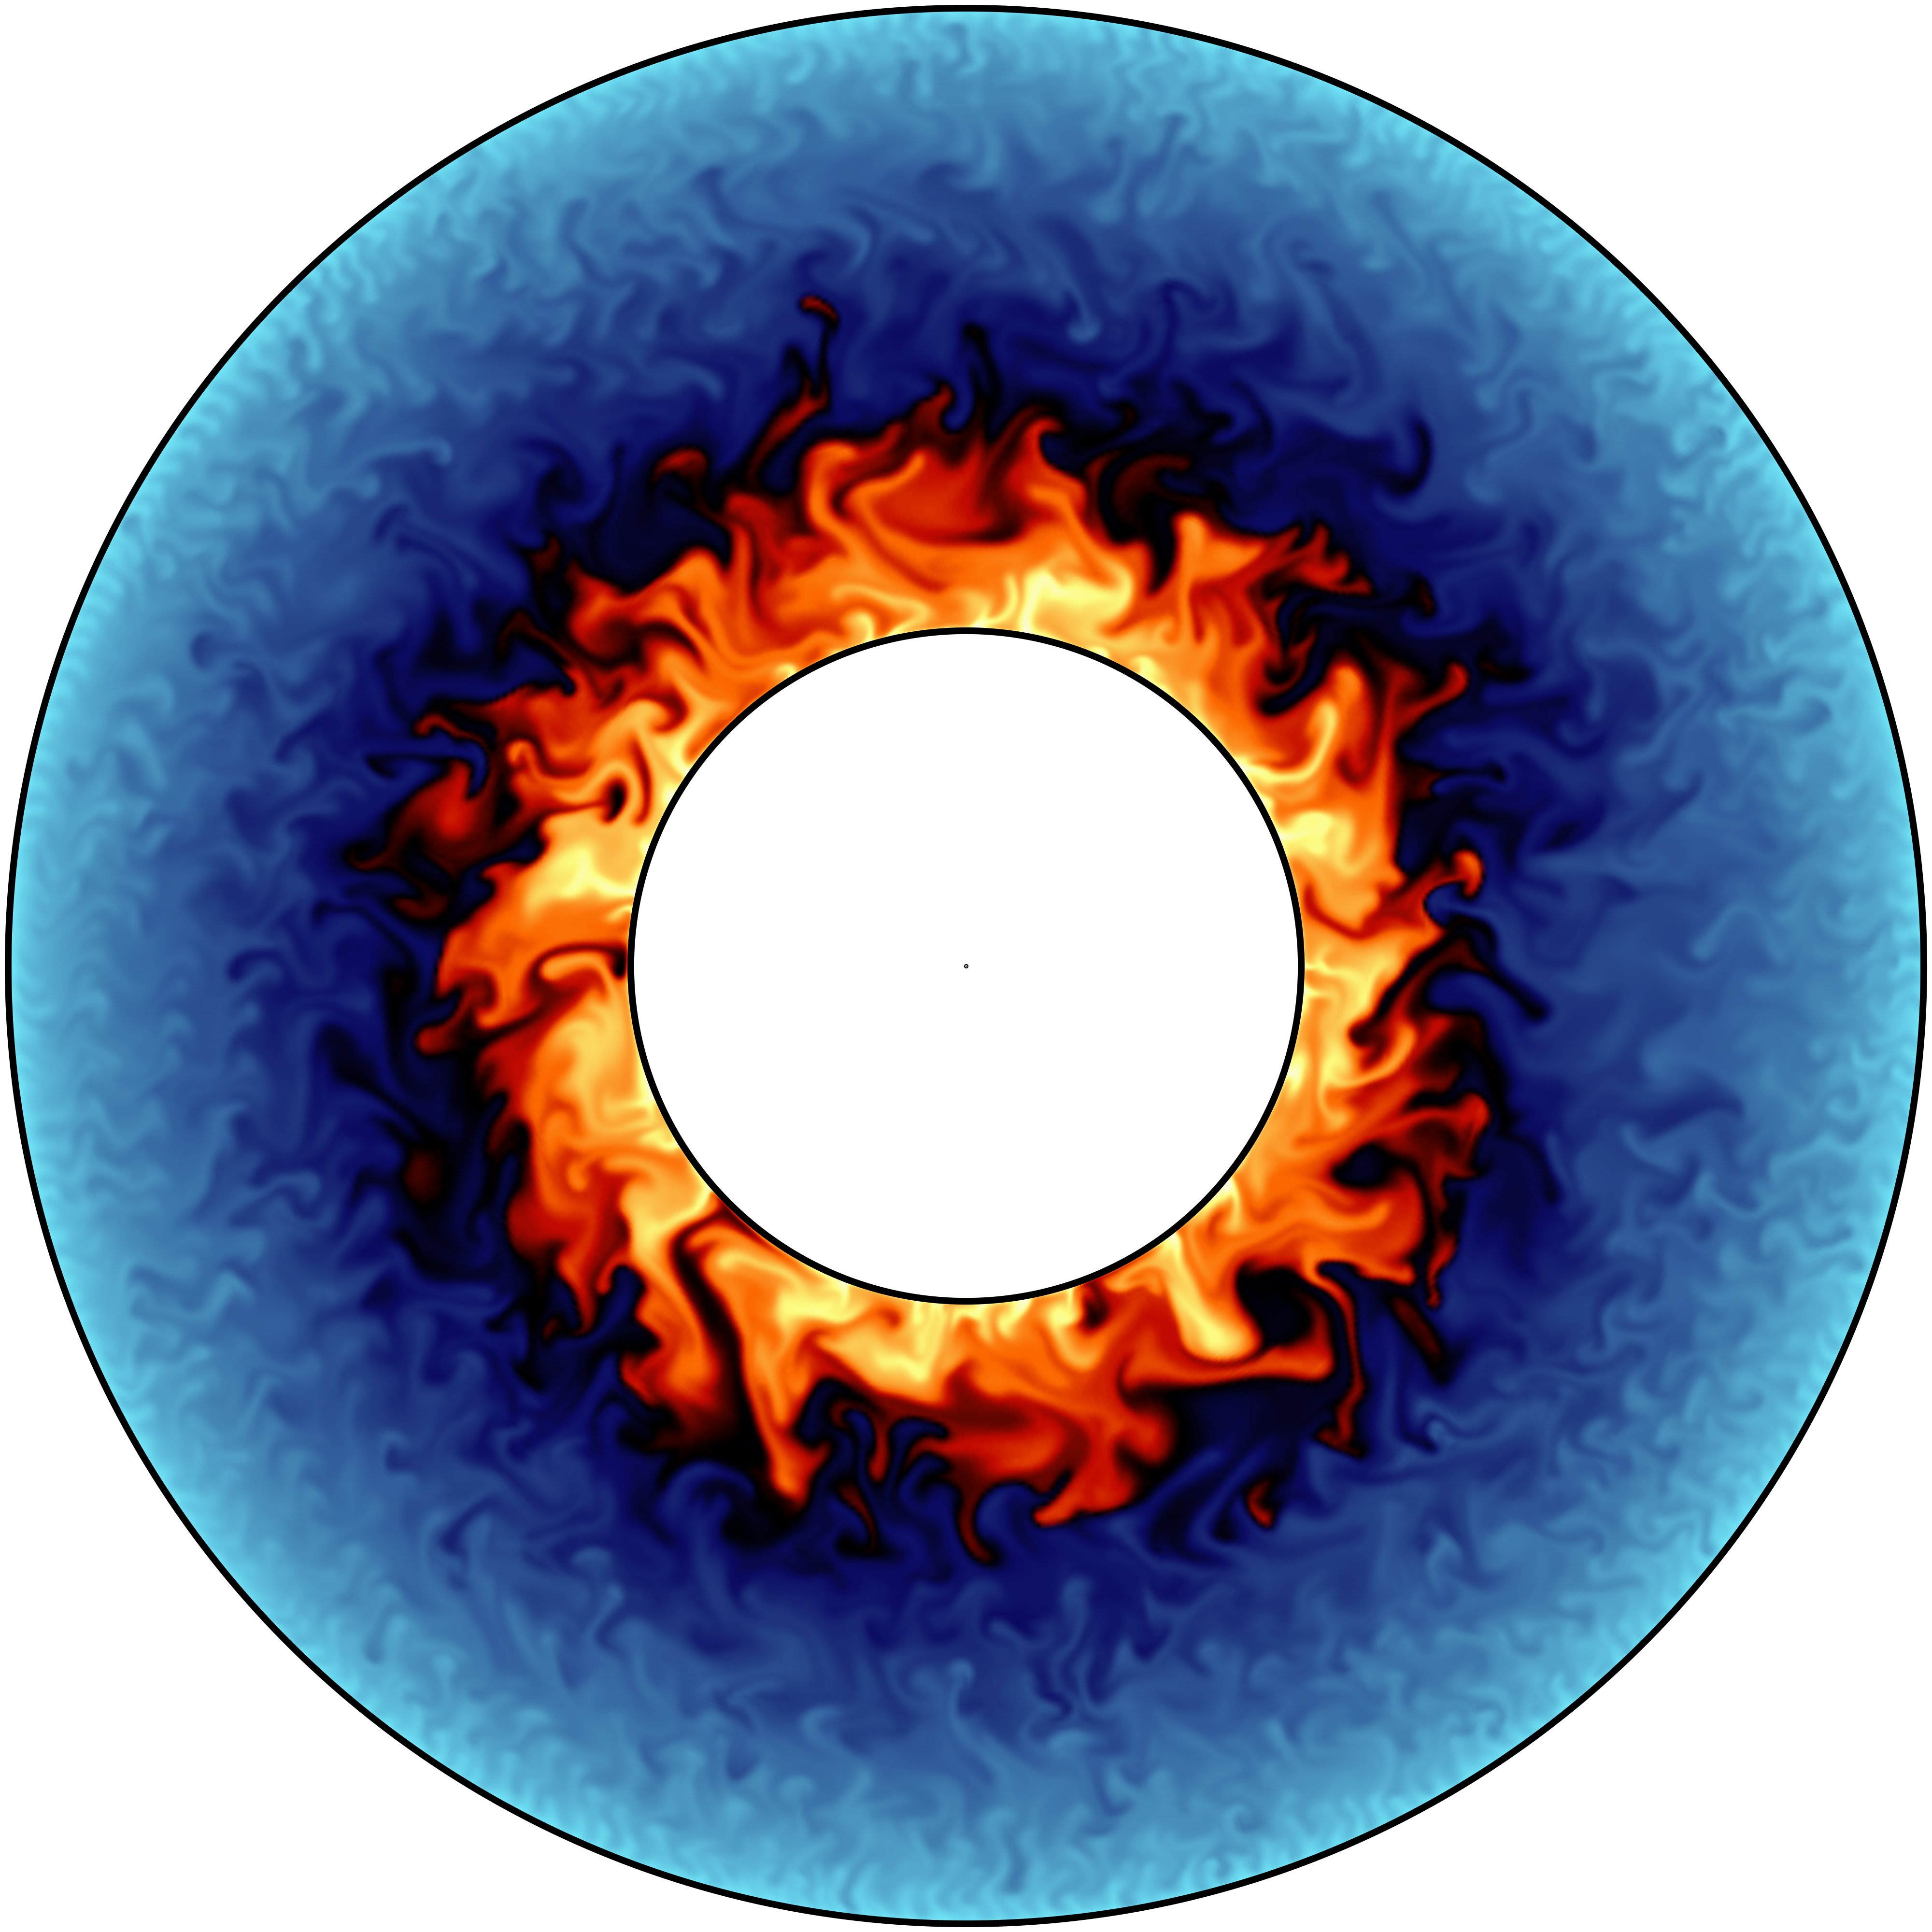
\includegraphics[width=0.25\textwidth]{figures/conv}}
	\end{center}
	\caption{(a) Artist interpretation of subsurface ocean on Europa, not to scale (NASA/JPL-Caltech). (b) Simulation (by author) of thermal convection in a planetary core\citep{tO25}.}
	\label{f:pic}
\end{wrapfigure}
The dynamics of these oceans are poorly understood, and neither EC nor JUICE will be able to make direct observations of the oceans. 
Therefore, forward numerical simulations are necessary to understand the interior dynamics. 
Furthermore, the coupling processes between the ocean and icy surface needs to be studied in order to make predictions that can be verified by the upcoming missions.
Current constraints on the thickness of Europa's ice shell, for example, range between $5-30$ km \citep{sV18}, but EC is expected to significantly reduce this uncertainty as well as provide spatially varying temperature profiles of the surface \citep{kS20}. 
Observations such as these will hint at the ocean dynamics, but only through processes not currently understood. In order to make the best use of EC and JUICE, it is necessary to have models that allow us to extrapolate surface measurements down to the oceans.
Indeed, a better understanding of coupled ice-ocean studies is one of the key future issues outlined in the most recent review of icy moon oceanography \citep{kS24}. 

I propose to  investigate forward, hydrodynamical models in which the coupling between the liquid ocean and icy surface is included. Two different coupling mechanisms will be studied. 
First, a conjugate heat transfer (CHT) model, in which the time-varying temperature profile in the icy shell is solved, will be built and run, which will provide new insight into the surface response to the underlying convection. Second, the double diffusion process, in which the bouyancy effects of both temperature and salinity are accounted for, will be investigated in the context of the ice-ocean boundary. Both studies will use 3D forward models of rotating convection in full spherical shells. 
\section{Background}
Europa, Callisto, and Ganymede, as well as the Saturnian moons Enceladus and Triton, were identified as likely ocean worlds after data began to return from the \textit{Galileo} and \textit{Cassini} missions \citep{fN16}.
Both gravity and magnetic measurements aided in the discovery, but in the case of Europa, the latter proves more convincing. 
Since the magnetic dipole of Jupiter is tilted about $10^{\circ}$ with respect to the orbital plane, the Jovian moons experience a magnetic induction as they orbit the planet.
Induced magnetic fields were measured by \textit{Galileo}, and it has been determined that a conducting ocean near the surface is likely necessary to explain observations\citep{fN16,cZ00}. 

It is likely that the oceans are turbulent and capable of convecting a large amount of heat and chemicals between the solid interior and icy crust.
A variety of forcing mechanisms have been proposed and discussed, such as electromagnetic coupling\citep{cGlP19}, tides, and precession\citep{kS24}, and in this investigation I propose to study buoyantly driven flows, in which variations in the fluid density drive convection.
Density variations are usually attributed to two separate effects-- thermal and compositional heterogeneities.
Thermally driven flows can be driven by radiogenic heating from the silicate core \citep{kS14,kS19,jK22} or tidal heating \citep{gT03,dL23}, which results in heterogeneous thermal forcing and may explain lateral variations in ice shell thickness. 
Compositional buoyancy is usually discussed in the context of salt fluxes near the outer boundary. 
Freezing (melting) can increase (decrease) salinity. The associate density variations drives convection and References \citep{yA21,wK22} predict that this mechanism serves to flatten the ice shell of Europa (ie.  homogenous thickness). 
\subsection{Non-dimensional parameters and flow regimes}
%\begin{figure}
%	\begin{center}
%		\subfloat[][]{
%		\includegraphics[width=0.66\textwidth]{figures/reg_diagram}
%	}
%		\quad
%		\subfloat[][]{
%		\includegraphics[width=0.22\textwidth]{figures/cht}
%	}
%	\end{center}
%	\caption{(a) Regime diagram for rotating convection, adapted from \citep{dL23,tG16}. The region left of the solid black line represent DNS results at $Pr = 1$ for a Europa-like geometry\citep{aB22}. The region right of the black line represents scaling predictions from \citep{tG16}. Dashed lines represent extrapolations of asymptotic predictions into the DNS region. Crosses and stars give the parameter space of modern simulations from Lemasquerier et al. 2023\citep{dL23} and Soderlund 2019\citep{kS19} respectively. Regions enclosed by dotted lines represent approximate parameter space for Europa and Ganymede \citep{dL23,kS19}. Red markers indicate proposed simulations for conjugate heat transfer (CHT) study.
%		(b) Schematic for CHT model.
%	}
%	
%	\label{f:reg_d}
%\end{figure}
\begin{figure}
	\begin{center}
		\includegraphics[width=0.7\textwidth]{figures/reg_diagram}
		\phantom{Lorem ipsum dolor sit amet}
	\end{center}
	\caption{Regime diagram for rotating convection, adapted from \citep{dL23,tG16}. The region left of the solid black line represent DNS results at $Pr = 1$ for a Europa-like geometry\citep{aB22}. The region right of the black line represents scaling predictions from \citep{tG16}. Dashed lines - extrapolations of asymptotic predictions into the DNS region. Crosses and stars - parameter space from Lemasquerier et al. 2023\citep{dL23} and Soderlund 2019\citep{kS19} respectively. Regions enclosed by dotted lines represent approximate parameter space for Europa and Ganymede \citep{dL23,kS19}. Red markers indicate proposed simulations for conjugate heat transfer (CHT) study.
	}
	\label{f:reg_d}
\end{figure}
There is a large disparity between the scales relevant to planetary bodies and the scales that can be realistically simulated.
%In simulating geophysical flows, there is often a large disparity between the spatial and temporal scales relevant to planetary bodies, and the scales that we can realistically compute. 
Usually this issue is formalized in terms of non-dimensional numbers that reflect ratios of the magnitudes of forcing mechanisms. %Alterntively, we can think of these quantities as ratios of different forcing terms in the governing equations. 
%In a geophysical and astrophysical context, there are two non-dimensional numbers of particular importance: the Rayleigh and Ekman numbers. 
The Rayleigh number $Ra$ describes the ratio of buoyancy to diffusivity. For planetary bodies, $Ra$ is very large, generally indicating vigourous convection.
The Ekman number $Ek$ approximates the ratio of viscous diffusion to Coriolis effects. Values for $Ek$ tend to be very small, indicating that rotation plays a dominant role.
Two other quantities of importance are the Nusselt number, $Nu$, and Prandtl number, $Pr$. 
They are the ratio of total heat transfer to conductive heat transfer and the ratio of momentum to thermal diffusivity respectively \citep{kS19}. 
Explicitly, these parameters are
\[Ra = \frac{g\alpha\Delta T D^{3}}{\nu\kappa_{T}}\quad Ek = \frac{\nu}{\Omega D^{2}} \quad Nu = \frac{hD}{k_{O}} \quad Pr= \frac{\nu}{\kappa_{T}},\]
where $g$ is the surface gravitational acceleration, $\alpha$ is the coefficient of thermal expansion, $D$ is the ocean thickness, $\nu$ and $\kappa_T$ are the diffusivities of momentum and temperature respectively, $\Omega$ is the planetary rotation rate, $h$ is the total heat transfer, and $k_O$ is the thermal conductivity of the ocean. $\Delta T$ indicates the temperature between the ocean surface and floor. 
A compositional Rayleigh number $Ra_{S}$ can be defined by replacing $\alpha, \Delta T,\text{ and, }\kappa_{T}$ with the associated quantities for salinity.
%Definitions and approximate values of these parameters are given in table \ref{t:nondim}.
%\begin{table}
%\begin{center}
%\begin{tabular}{|c|c|c|c|c|c|c|}
%\hline
%Values&$Ra$ &$Ek$ &$Nu$ & $Pr$ &$Bi$ &$Le$\\
%\hline
%Definition&$\frac{g\alpha\Delta T D^{3}}{\nu\kappa_{T}}$& $\frac{\nu}{D^{2}\Omega}$ %Ra,Ek
%	  &$\frac{hD}{k_o}$ &$\frac{\nu}{\kappa_{T}}$ %Nu,Pr
%	  &$\frac{hD_i}{k_{i}}$ &$\frac{\kappa_{T}}{\kappa_{S}}$\\%Bi,Le
%	  \hline
%\end{tabular}
%\end{center}
%\caption{Definitions of non-dimensional parameters. $g$ is the surface gravitational acceleration, $\alpha$ is the coefficient of thermal expansion, $D$ is the ocean thickness, $\nu$ and $\kappa$ are the diffusivities of momentum and temperature respectively, $\Omega$ is the planetary rotation rate, $h$ is the total heat transfer, and $k_o(i)$ is the thermal conductivity of the ocean (ice). $\Delta T$ indicates the temperature between the ocean surface and floor. Approximate values for icy moons shown in figure \ref{f:reg_d}}.
%\label{t:nondim}
%\end{table}
%\begin{SCtable}[50]%{l}{5.5cm}
%	%\begin{adjustbox}{minipage=\linewidth,bgcolor={gray_c}}
%%\begin{tabular}{|c|c|}
%	\large
%\begin{tblr}{
%    colspec = {|c|c|},
%    row{1} = {gray_h},
%    row{2-7} = {gray_c},
%  }
%\hline
%Parameter&Definition\\%$Ra$ &$Ek$ &$Nu$ & $Pr$ &$Bi$ &$Le$\\
%\hline
%$Ra$&$\frac{g\alpha\Delta T D^{3}}{\nu\kappa_{T}}$\\
%\hline
%$Ek$ &$\frac{\nu}{D^{2}\Omega}$\\
%\hline
%$Nu$&$\frac{hD}{k_O}$\\
%\hline
%$Pr$&$\frac{\nu}{\kappa_{T}}$\\
%\hline
%$Bi$ &$\frac{hD_i}{k_{i}}$\\
%\hline
%$Le$ &$\frac{\kappa_{T}}{\kappa_{S}}$\\
%\hline
%%\end{tabular}
%\end{tblr}
%\caption{Definitions of non-dimensional parameters. $g$ is the surface gravitational acceleration, $\alpha$ is the coefficient of thermal expansion, $D$ is the ocean thickness, $\nu$ and $\kappa$ are the diffusivities of momentum and temperature respectively, $\Omega$ is the planetary rotation rate, $h$ is the total heat transfer, and $k_o(i)$ is the thermal conductivity of the ocean (ice). $\Delta T$ indicates the temperature between the ocean surface and floor. Approximate values for icy moons shown in figure \ref{f:reg_d}.}
%\label{t:nondim}
%%\end{adjustbox}
%
%\end{SCtable}

To take Europa as an example, predicted values of $Ra$ and  $Ek$ are $O\lb 10^{20}\rb $ and $O\lb 10^{-12}\rb $ respectively. Modern direct numerical simulations (DNS) have only reached values of $Ra \sim 10^{8}$ and $Ek \sim 10^{-5}$\citep{dL23}. In studies of different planetary bodies, more aggressive simulations have been performed (eg. figure \ref{f:pic}(b), references \citep{cG19,tG16,tO25}), however all fall significantly short of reaching realistic values. For icy moons, it is particularly difficult to reach small values of $Ek$ because the ocean depth is much smaller than the planetary radius. The procedure, therefore, is to attempt to establish scaling laws with the non-dimensional parameters by simulating at moderate values, and then extrapolating to planetary values.

It is insufficient to establish scaling relations for each non-dimensional parameter independently. 
%Flow behaviours can vary wildly depending on the particular combination of the non-dimensional parameters. 
For example, at a value of $Ra = 10^{8}$ a non-rotating flow ($Ek\rightarrow \infty$) is expected to vigourously convect, however rapid rotation (low  $Ek$) will stifle and change the structure of the convection, or even arrest it entirely\citep{sC61}. 
Figure \ref{f:reg_d} displays a cross-section of $Ek,Ra$ parameter space, and recognized convective regimes \citep{tG16}. The ordinate is $RaEk^{4/3},$ which determines the boundary between conduction and convection\citep{sC61}.

As $Ek\rightarrow 0$, rotational effects dominate the system and suppress radial motion. The ``conductive,'' ``weakly non-linear,'' and ``rapidly rotating'' regimes\citep{tG16,kJ12} are all characterized by axially stretched flows conforming to the Taylor-Proudman (TP) theorem at leading order. TP dictates that rapidly-rotating flows remain invariant along the axis of rotation \citep{gB53}.
%As $Ra$ is increased, convection sets in as axially stretched flows conforming to the Taylor-Proudman theorem \citep{gB53}, which dictates that rapidly-rotating flows remain invariant along the axis of rotation. Such dynamics are known as geostrophic.
%Geostrophic flows are laminar over a small range of $Ra,$ but quickly become turbulent. Geostrophy holds over large time and length scales, but on small scales low order fluctuations make the dynamics highly non-linear.
%This regime is often referred to as ``rapidly rotating'' or ``geostrophic turbulence'' \citep{kJ12}.

Further increase of $Ra$ yields the ``transitional" regime, where the TP constraint is significantly relaxed, but flows are still rotationally influenced.
Eventually, flows become turbulent enough that rotation's role is minimal. This regime is labeled ``non-rotating.''
Although significant uncertainty exists, it is believed that the icy-moons lie in the transitional and non-rotating regimes\citep{dL23,tG16}.

Forward models in this regime\citep{kS19, dL23}, have investigated only the ocean domain. The fixed melting temperature of ice is prescribed at the fluid domain boundary.
%and have prescribed boundary conditions at the ocean-ice interface to represent the fixed melting temperature of the ice. 
A forward model with a melting icy boundary was used to constraing ice topography, but the fast timescale heat fluctuations in the icy shell were not investigated\citep{jK24}.

%A model with a dynamic, melting icy boundary has been studied, however the authors were primarily interested in the resulting topography. The fast timescale heat fluctuations in the icy shell due to the underlying convection were not investigated\citep{jK24}. 

CHT is a simulation configuration in which a solid boundary is included in the solution domain so that heat is able to conduct from the fluid into the boundary. Rather than placing a boundary condition on the fluid surface, the condition is placed on the outermost solid surface and the liquid and solid domains are solved together\citep{dA09}. Whether CHT is important can be estimated by the value of the Biot number $Bi$ \citep{dA09,jL24}, a non-dimensional parameter representing the ratio of conductive resistance to convective heat flow. For the conjugate problem, $Bi$ can be estimated as
\[Bi \sim Nu\frac{k_{f}}{k_{i}}\frac{D_{i}}{D},\]
where $k_{f\lb i\rb }$ is the thermal conductivity of the fluid (ice) and $D_{i}$ is the ice depth.
Estimates for Europa therefore suggest $Bi \sim O\lb 10^{6}\rb$\citep{dL23}. When $Bi>1,$ the conjugate problem is considered relevant, and therefore this process likely plays a role in the evolution of icy shells.
\subsection{Compositional convection}
%On Earth, salinity is known to play an important role in oceanic convection. Salt fingering is regularly observed in terrestial oceans\citep{jT73} and is understood to result from the interaction between a stable temperature gradient and unstable salinity gradient. The freezing and melting of sea ice. 

The electrical conductive properties of the Jovian satellites likely imply salty oceans\citep{cZ00}.
%which suggests a variety of consequences. At pressures relevant to the icy moons, salinity can reverse the sign of the thermal expansivity coefficient $\alpha$ at temperatures close to, but greater than, the melting temperature. This means that colder fluid is less dense, which may allow for the generation of a buoyantly stable layer that inhibits heat and mass transport \citep{aT64}. 
%Furthermore, 
Salinity affects fluid density even in the absence of temperature variations which provides a second source of buoyancy. 
%This mechanism provides a second source of buoyancy and can yield double diffusive convection (DDC). 
Because the molecular diffusivities of salt and temperature are different, stably stratified fluids may be convectively unstable. 
This gives rise to double diffusive convection (DDC)\citep{sK66,tR13}.
This instability is fundamentally diffusive, which necessitates the use of molecular (rather than turbulent) values of diffusivity.
The ratio of diffusivities $\kappa_T/ \kappa_S=Le$ is the Lewis number, and, based on terrestial values, is $O(10^2)$.

On Earth, sea ice often provides a reservoir of cold, fresh water at the ocean surface. 
Warmer, salty water underneath yields an unstable temperature gradient and stable salinity gradient, which can lead to long-lived layers of fluid separated by diffusive boundaries which control vertical transport \citep{mT08,jT73,jT02}. 
In simulations, rotation is known to prolong the existence of these layers compared to the non-rotating case \citep{jF24}.
%This situation has been studied extensively in the terrestial ocean context\citep{jT73,jT02}, although the application to icy moons is not clear. The primary difference is that relative to the planetary radius, the ocean depth for the icy moons is significantly greater than Earth's oceans, which has significant implications for the effects of rotation.
The DDC problem is numerically expensive, and the studies above, as well as many others, have primarily used plane layers. In rotating studies, constant rotation vectors are used\citep{gM12,rM17}.  
Reference \citep{rM19} simulated a spherical shell and determined that the primary convective instability is inviscid, which suggests that double diffusive systems may be significantly more turbulent than purely thermal systems at similar parameter regimes. However they considered the case where salinity gradients are unstable and temperature gradients are stable; the situation opposite what is expected for icy moons.

A global ciruclation model for icy moons was simulated in reference \citep{yA21}. They suggest that salinity is the dominant source of buoyancy in Europa, and that the convection should serve to homogenize the ice shell thickness. However, $Le=1$ (ie. equal thermal and compositional diffusivity) which means that instabilities associated with DDC are not included in the study.

\section{Proposed project and methodology}
I propose two sets of simulations in order to study ice-ocean coupling in the icy moons. The first study will involve the CHT model and will be performed within the state of the art parameter regimes previously reported by references\citep{dL23,kS19} (which do not involve the CHT framework).
The second study will focus on DDC. The proposed simulations are listed in table \ref{t:param}.
\subsection{Conjugate heat transfer}
\begin{table}
\begin{center}
\begin{tabular}{|c|c|c|c|c|c|c|}
\hline
Model&Geometry&$Ra$&$Ek$&$D/D_{i}$ or $Ra_S$ &\# Simulations & Cost (cpu$\times$hour)\\
\hline
CHT& Shell&$\lb 5 \times 10^{6} - 2 \times 10^{8} \rb $ & $3 \times 10^{-4} $ & $2,10$&10&$7 \times 10^{5}$\\
\hline
CHT& Shell&$\lb 5 \times 10^{6} - 1 \times 10^{9} \rb $ & $1 \times 10^{-4} $ & $2,10$&10&$1\times 10^{6}$\\
\hline
CHT& Shell&$\lb 5 \times 10^{7} - 2 \times 10^{9} \rb $ & $3 \times 10^{-5} $ & $2,10$&10&$2\times 10^6$\\
\hline
DDC& Shell & $10^5$& $\infty$&$10^4-10^5$& 5& $2\times 10^{6}$\\
\hline
DDC& Shell & $10^5$& $10^{-4}$&$10^4-10^5$& 5& $2\times 10^{6}$\\
\hline
DDC& Plane &$5\times10^{5}-2\times10^{6}$ & $3\times10^{-4}$&$12.5Ra$ &5 &$2.5\times 10^{5}$  \\
\hline
DDC& Plane &$10^{6}-10^{7}$ & $10^{-4}$&$12.5Ra$& 5 & $5\times 10^{5}$\\
\hline
DDC& Plane &$10^{7}-5\times 10^{7}$ & $3\times10^{-5}$&$12.5Ra$ & 5& $10^{6}$ \\
\hline
Totals & & & & & 55&$9.5 \times 10^6$ \\
\hline
\end{tabular}
\end{center}
\caption{Proposed parameter space. The fifth column presents the ratio of ocean to ice thicknesses for the CHT model and the compositional Rayleigh number for the DDC model. 
Computing costs are estimate values based off of existing studies \citep{rM19,rM17,dL23,jF24} and personal experience with relevant codes.}
\label{t:param}
\end{table}
I will explore Boussinesq convection in a thin, liquid shell surrounded by a thermally conducting layer. 
In particular, I will perform a sweep of $30$ simulations across parameter space (see table \ref{t:param}, figure \ref{f:reg_d}) and extrapolate the results to regimes associated with icy moons.
At larger values of $Ek,$ I will simulate the transitional and non-rotating regimes, however at the smallest $Ek$ values, I intend to focus on the transitional regime in order to better compare with existing studies and reduce computational cost.
The hydrodynamic code \texttt{Nek5000}\citep{nek5000} is capable of solving the CHT problem and I have already used the code extensively to solve related geophysical problems. 
Based on the numerical resolutions reported in \citep{dL23}.

Primarily I will report temperature distributions within the icy shell. I will also investigate global transport quantities, such as convected heat, and structural quantities, such as latitudinal profiles of temperature. 
These latter results can be compared to existing studies \citep{dL23,kS19,jK22} to determine whether the CHT setup has significant effects on the convection itself.
\subsection{Double diffusive convection}
I will investigate double-diffusive convection (DDC) in a non-rotating and slowly rotating (moderate $Ek$) context. Due to the significant computational constraints, I propose to study a spherical shell geometry for only non-rotating and slowly rotating ($Ek = 10^{-4}$) flows. I will supplement these results with a suite of local, rotating simulations in cartesian plane layers. Previously, cartesian simulations for purely thermal convection on the icy moons have been used in which a complete treatment of the Coriolis effect is employed \citep{sB22}. I propose to use the same model setup, but include DDC effects. 
Because DDC yields diffusive instabilities, I will investigate molecular values of diffusivity rather than turbulent values used in \citep{sB22}. Therefore, simulations need be performed at more moderate values of $Ek, Ra$. 
All simulations will be performed at $Le = 10$ and $Pr = 1$. 
The chosen parameter values are intended to remain in the transitional regime without necessesitating exorbitant computation. They are based off of previous studies of DDC in Jupiter\citep{jF24,rM17}. 
My primary focus will be to investigate the formation of distinct layers often seen in DDC.
Layered structures can control transport, which means that their formation and structure may play a key role in the interaction between the ocean and surface ice. This process is poorly understood and numerical simulations are necessary to understand the ocean dynamics. 
\subsection{Computing requirements}
In total, I plan to conduct $55$ numerical experiments, which I estimate to require $9.5\times 10^{6}$ cpu-hours. I will apply for computing time through ACCESS and TACC, which are both supported by the National Science Foundation. I will also apply for local computing resources depending on the host institution.
\begin{spacing}{0.4}
\begin{multicols}{2}
%\bibliography{References,journal_abbreviations}%jfm-bib,References}

\printbibliography

\end{multicols}
\end{spacing}
\end{document}
